\chapter{Convolutions beyond images}
\label{chap:convolutions_beyond_images}

\begin{supportbox}{About this chapter}
Convolutional models are a powerful baseline model in many applications, going far beyond image classification. In this chapter we provide an overview of several such extensions, including the use of convolutional layers for 1D and 3D data, text modeling, and autoregressive generation. Several of the concepts we introduce (e.g., masking, tokenization) are fundamental in the rest of the book.
\end{supportbox}

\section{Convolutions for 1D and 3D data}
\subsection{Beyond images: time series, audio, video, text}

In the previous chapter we focused exclusively on images. However, many other types of data share similar characteristics, i.e., one or more “ordered” dimensions representing time or space, and one dimension representing features (the channels in the image case). Let us consider some examples:
%
\begin{enumerate}
\item \textbf{Time series} are collections of measurements of one or more processes (e.g., stocks prices, sensor values, energy flows). We can represent a time series as a matrix $\mathbf{X} \sim (t,c)$, where $t$ is the length of the time series, and $\mathbf{X}_i \sim (c)$ are the $c$ measurements at time $t$ (e.g., $c$ sensors from an EEG scan, or $c$ stock prices). Each time instant is equivalent to a pixel, and each measurement is equivalent to a channel.
\item \textbf{Audio} files (speech, music) can also be described by a matrix $\mathbf{X} \sim (t,c)$, where $t$ is now the length of the audio signal, while $c$ are the channels of the recording ($1$ for a mono audio, $2$ for a stereo signal, etc.). 
%
\begin{supportbox}{Frequency-analysis}
    Audios can also be converted to an image-like format via frequency analysis (e.g., extracting the MFCC coefficients over small windows), in which case the resulting \textit{time-frequency} images represent the evolution of the frequency content over the signal - see Figure \ref{fig:audio_analysis_frequency} for an example. With this preprocessing we can use standard convolutional models to process them.
\end{supportbox}
    %
    \item \textbf{Videos} can be described by a rank-$4$ tensor $X \sim (t, h, w, c)$, where $t$ is the number of \textit{frames} of the video, and each frame is an image of shape $(h,w,c)$. Another example is a volumetric scan in medicine, in which case $t$ is the volume depth.
\end{enumerate}

\begin{figure}
    \centering
    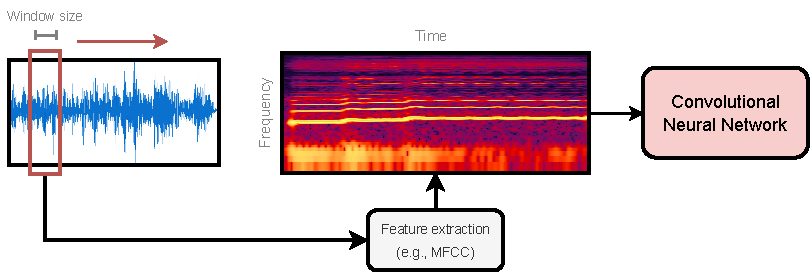
\includegraphics[width=1.0\textwidth]{images/audio_classification_CNN}
    \caption{Audio can be represented as either a 1D sequence (left), or a 2D image in a time-frequency domain (middle). In the second case, we can apply the same techniques described in the previous chapter.}
    \label{fig:audio_analysis_frequency}
\end{figure}

Time series, audio signals, and videos can be described by their \textbf{sampling rate}, which denotes how many samples are acquired per unit of time, sometimes expressed in samples per second, or hertz (Hz). For example, classical EEG units acquire signals at 240 Hz, meaning 240 samples each second. A stock can be checked every minute, corresponding to 1/60 Hz. By contrast, audio is acquired with very high frequency to ensure fidelity: for example, music can be acquired at $44.1e^3$ Hz (or $44.1$ kHz). Typical acquisition \textbf{frame rates} for video are instead around $24$ frames per second (fps) to ensure smoothness to the human eye.

Image resolution, audio sampling rate, and video frame rates all play similar roles in determining the precision with which a signal is acquired. For an image, we can assume a fixed resolution a priori (e.g., $1024 \times 1024$ pixels). This is reasonable, since images can always be reshaped to a given resolution while maintaining enough consistency, except for very small resolutions. By contrast, audio and video durations can vary from input to input (e.g., a song of 30 seconds vs. a song of 5 minutes), and they cannot be reshaped to a common dimension, meaning that our datasets will be composed of \textbf{variable-length} data. In addition, audio resolution can easily grow very large: with a $44.1$ kHz sampling rate, a $3$-minute audio will have $\approx 8M$ samples.

We also note that the dimensions in these examples can be roughly categorized as either “spatial dimensions” (e.g., images) or “temporal dimensions” (e.g., audio resolution). While images can be considered symmetric along their spatial axes (in many cases, an image flipped along the width is another valid image), time is \textit{asymmetric}: an audio sample inverted on its temporal axis is in general invalid, and an inverted time series represents a series evolving from the future towards its past. Apart from exploiting this aspect in the design of our models (\textbf{causality}), we can also be interested in \textit{predicting} future values of the signal: this is called \textbf{forecasting}.

Finally, consider a text sentence, such as “\textit{the cat is on the table}”. There are many ways to split this sentence into pieces. For example, we can consider its individual syllables: [”\textit{the}”, “\textit{cat}”, “\textit{i}”, “\textit{s}”, “\textit{on}”, “\textit{the}”, “\textit{ta}”, \textit{ble}”]. This is another example of a sequence, except that each element of the sequence is now a categorical value (the syllable) instead of a numerical encoding. Hence, we need some way of encoding these values into features that can be processed by the model: splitting a text sequence into components is called \textbf{tokenization}, while turning each token into a vector is called \textbf{embedding} the tokens.

In the next sections we consider all these aspects (variable-length inputs, causality, forecasting, tokenization, and embedding) in turn, to see how we can build convolutional models to address them. Some of the techniques we introduce, such as masking, are very general and are useful also for other types of models, such as transformers. Other techniques, such as dilated convolutions, are instead specific to convolutional models.

\subsection{1D and 3D convolutional layers}

Let us consider how to define convolutions for 1D signals (e.g., time series, audio) and their extension to 3D signals (e.g., videos). Note that the dimensionality refers only to the number of dimensions along which we convolve (spatial or time), and does not include the channel dimension. Recall that, in the 1D case, we can represent the input as a single matrix:

\vspace{1em}
\begin{equation*}
\mathbf{X} \sim (\eqnmarkbox[drawred]{node}{t}, \eqnmarkbox[drawgreen]{node2}{c})
\end{equation*}
\annotate[yshift=-1em]{below,left}{node}{Length of the sequence}
\annotate[yshift=-1em]{below,right}{node2}{Features}

\vspace{1em}
We now replicate the derivation from Chapter \ref{chap:cnns}. Given a patch size $s=2k+1$, we define $P_{k}(i) \sim (s,c)$ as the subset of rows in $\mathbf{X}$ at distance at most $k$ from $i$ (ignoring border elements for which zero-padding can be used). A 1D convolutional layer $\mathbf{H} = \text{Conv1D}(\mathbf{X})$ outputs a matrix $\mathbf{H} \sim (t, c^\prime)$, with $c^\prime$ an hyper-parameter that defines the output dimensionality, defined row-wise as:
%
\begin{equation}
\idx{\text{Conv1D}(X)}{i} = \phi(\mathbf{W} \cdot\text{vect}(P_{k}(i)) + \mathbf{b})
\label{eq:1d_convolution}
\end{equation}
%
with trainable parameters $\mathbf{W} \sim (c^\prime,sc)$ and $\mathbf{b} \sim (c^\prime)$. Like in the 2D case, this layer is local (for a properly modified definition of locality) and equivariant to translations of the sequence. 

In the 2D case, we also discussed an alternative notation with all indices explicitly summed over:
%
\begin{equation}
H_{ijz} = \sum_{i^\prime=1}^{2k+1}\sum_{j^\prime = 1}^{2k+1}\sum_{d=1}^{c} \idx{W}{i^\prime, j^\prime,z,d}\idx{X}{i^\prime+t(i),j^\prime+t(j),d}
\label{eq:conv_again}
\end{equation}
%
where $t(i)=i+k-1$ as in \eqref{eq:convolutive_offset}. Recall that we use $t$ to index $i^\prime$ and $j^\prime$ differently for the two tensors: from $1$ to $2k+1$ for $W$, and from $i-k$ to $i+k$ for $X$. The equivalent variant for \eqref{eq:1d_convolution} is obtained trivially by removing one summation index:

\begin{equation}
H_{iz} = \sum_{i^\prime=1}^{2k+1}  \sum_{d=1}^{c} \idx{W}{i^\prime,z,d}\idx{X}{i^\prime+t(i),d}
\label{eq:1d_convolution_sum}
\end{equation}

where the parameters $W \sim (s, c^\prime, c)$ are now organized in a rank-$3$ tensor. By contrast, the 3D variant is obtained by adding a new summation over the third dimension with index $p$:

$$
H_{{\color{drawred}p}ijz} = {\color{drawred}\sum_{p^\prime=1}^{2k+1}}\sum_{i^\prime=1}^{2k+1}\sum_{j^\prime = 1}^{2k+1},\sum_{d=1}^{c} \idx{W}{{\color{drawred}p^\prime}, i^\prime, j^\prime,z,d}\idx{X}{{\color{drawred}p^\prime+t(p)},i^\prime+t(i),j^\prime+t(j),d}
$$

We assume that the kernel size is identical across all dimensions for simplicity. With similar reasonings we can derive a vectorized 3D variant of convolution, and also 1D and 3D variants of max pooling.


\section{Convolutional models for 1D and 3D data}

We now consider the design of convolutional models in the 1D case, with a focus on how to handle variable-length inputs and how to deal with text sequences. Several of the ideas we introduce are fairly generic for all differentiable models.


\subsection{Dealing with variable-length inputs}

Consider two audio files (or two time series, or two texts), described by their corresponding input matrices $\mathbf{X}_1 \sim (t_1, c)$ and $\mathbf{X}_2 \sim (t_2, c)$. The two inputs share the same number of channels $c$ (e.g., the number of sensors), but they have different lengths, $t_1$ and $t_2$. Remember from our discussion in Section \ref{sec:towards_convolutive_layers} that convolutions can handle (in principle) such \textbf{variable-length} inputs. In fact, denote by $g$ a generic composition of 1D convolutions and max-pooling operations, corresponding to the feature extraction part of the model. The output of the block are two matrices:
%
$$
\mathbf{H}_1=g(\mathbf{X}_1)\,,\,\mathbf{H}_2=g(\mathbf{X}_2)
$$
%
having the same number of columns but a different number of rows (depending on how many max-pooling operations or strided convolutions are applied on the inputs). After global average pooling, the dependence on the length disappears:
%
$$
\mathbf{h}_1=\sum_i\mathbf{H}_{1i} \,,\,\mathbf{h}_2=\sum_i\mathbf{H}_{2i}
$$
%
and we can proceed with a final classification on the vectors $\mathbf{h}_1$ and $\mathbf{h}_2$. However, while this is not a problem at the level of the model, it is a problem in practice, since mini-batches cannot be built from matrices of different dimensions, and thus operations cannot be easily vectorized. This can be handled by zero-padding the resulting mini-batch to the maximum dimension across the sequence length. Assuming for example, without lack of generality, $t_1 > t_2$, we can build a “padded” mini-batch as:
%
$$
X=\text{stack}\left(\mathbf{X}_1,\begin{bmatrix}\mathbf{X}_2\\ \mathbf{0}\end{bmatrix}\right)
$$
%
where $\text{stack}$ operates on a new leading dimension, and the resulting tensor $X$ has shape $(2, t_1,  c)$. We can generalize this to any mini-batch by considering the largest length with respect to all elements of the mini-batch. For a convolution, this is not very different from zero-padding, and operating on the padded input will not influence significantly the operation (e.g., in audio, zero-padding is equivalent to adding silence at the end).  See Box \ref{code:mini_batch_padding} for an example of building a padded mini-batch. 

\begin{mypy}{A padded mini-batch from three sequences of variable length (with $c=8$). When using a {\footnotesize\mintinline{python}{DataLoader}}, padding can be achieved by over-writing the default {\footnotesize\mintinline{python}{collate_fn}}, which describes how the loader concatenates the individual samples.}{code:mini_batch_padding}
# Sequences with variable length (3, 5, 2, respectively)
X1, X2, X3 = torch.randn(3, 8), 
             torch.randn(5, 8), 
             torch.randn(2, 8)

# Pad into a single mini-batch
X = torch.nn.utils.rnn.pad_sequence([X1, X2, X3], 
                    batch_first=True)
print(X.shape) # [Out]: torch.Size([3, 5, 8])
\end{mypy}

Alternatively, we can build a masking matrix describing valid and invalid indexes in the mini-batched tensor:
%
$$
\mathbf{M}=\begin{bmatrix} \mathbf{1}_{t_1} \\ \mathbf{1}_{t_2} \;\;\mathbf{0}_{t_1-t_2} \end{bmatrix}
$$
%
where the index denotes the size of the vectors. These masking matrices can be helpful to avoid invalid operations on the input tensor.

\subsection{CNNs for text data}

Let us consider now the problem of dealing with text data. As we mentioned previously, the first step in dealing with text is \textbf{tokenization}, in which we divide the text (a string) into a sequence of known symbols (also called \textbf{tokens} in this context). There are multiple types of tokenizers:
%
\begin{enumerate}
\item \textbf{Character tokenizer}: each character becomes a symbol.
\item \textbf{Word tokenizer}: each (allowed) word becomes a symbol.
\item \textbf{Subword tokenizer}: intermediate between a character tokenizer and a word tokenizer, each symbol is possibly larger than a character but also smaller than a word.
\end{enumerate}

\begin{SCfigure}
    \centering
    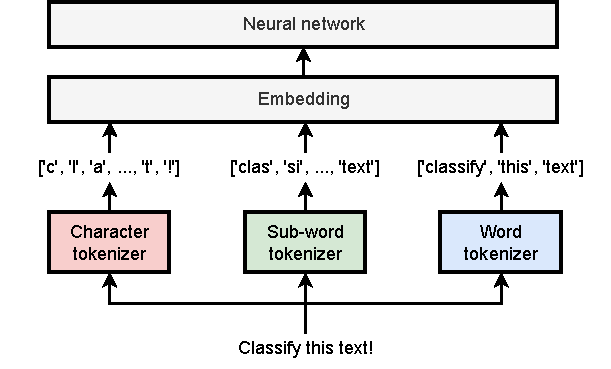
\includegraphics[width=0.7\textwidth]{images/text_tokenization}
    \caption{Starting from a text, multiple types of tokenizers are possible. In all cases, symbols are then embedded as vectors and processed by a generic 1D model.}
    \label{fig:text_tokenization}
\end{SCfigure}

This is shown schematically in Figure \ref{fig:text_tokenization}. In all three cases, the user has to define a \textbf{dictionary} (\textbf{vocabulary}) of allowed tokens, such as all ASCII characters for a character tokenizer. In practice, one can select a desired size of the dictionary, and then look at the most frequent tokens in the text to fill it up, with every other symbol going into a special “out-of-vocabulary” (OOV) token. Subword tokenizers have many specialized algorithms to this end, such as byte-pair encoding (BPE) \cite{shibata1999byte}.\footnote{This is a short exposition focused on differentiable models, and we are ignoring many preprocessing operations that can be applied to text, such as removing stop words, punctuation, “stemming”, and so on. As the size of the models has grown, these operations have become less common.}

Because large collections of text can have a wide variability, pre-trained subword tokenizers are a standard choice nowadays.  As a concrete example, OpenAI has released an open-source version of its own tokenizer,\footnote{\url{https://github.com/openai/tiktoken}} which is a subword model consisting of approximately 100k subwords (at the time of writing). Consider for example the encoding of “\textit{This is perplexing!}” with this tokenizer, shown in Figure \ref{fig:tiktoken}. Some tokens correspond to entire words (e.g., “\textit{This}”), some to pieces of a word (e.g, “\textit{perplex}”), while others to punctuation marks. The sequence can be equivalently represented by a sequence of integers:
%
\begin{equation}
[2028, 374, 74252, 287, 0]
\label{eq:list_of_indices}
\end{equation}
%
Each integer spans between $0$ and the size of the vocabulary (in this case, roughly 100k), and it uniquely identifies the token with respect to that vocabulary. In practice, nothing prevents us from adding “special” tokens to the sequence, such as tokens representing the beginning of the sentence (sometimes denoted as [BOS]), OOV tokens, or anything else. The [BOS] token will be of special significance in the next section.

\begin{SCfigure}
    \centering
    \hspace{1em}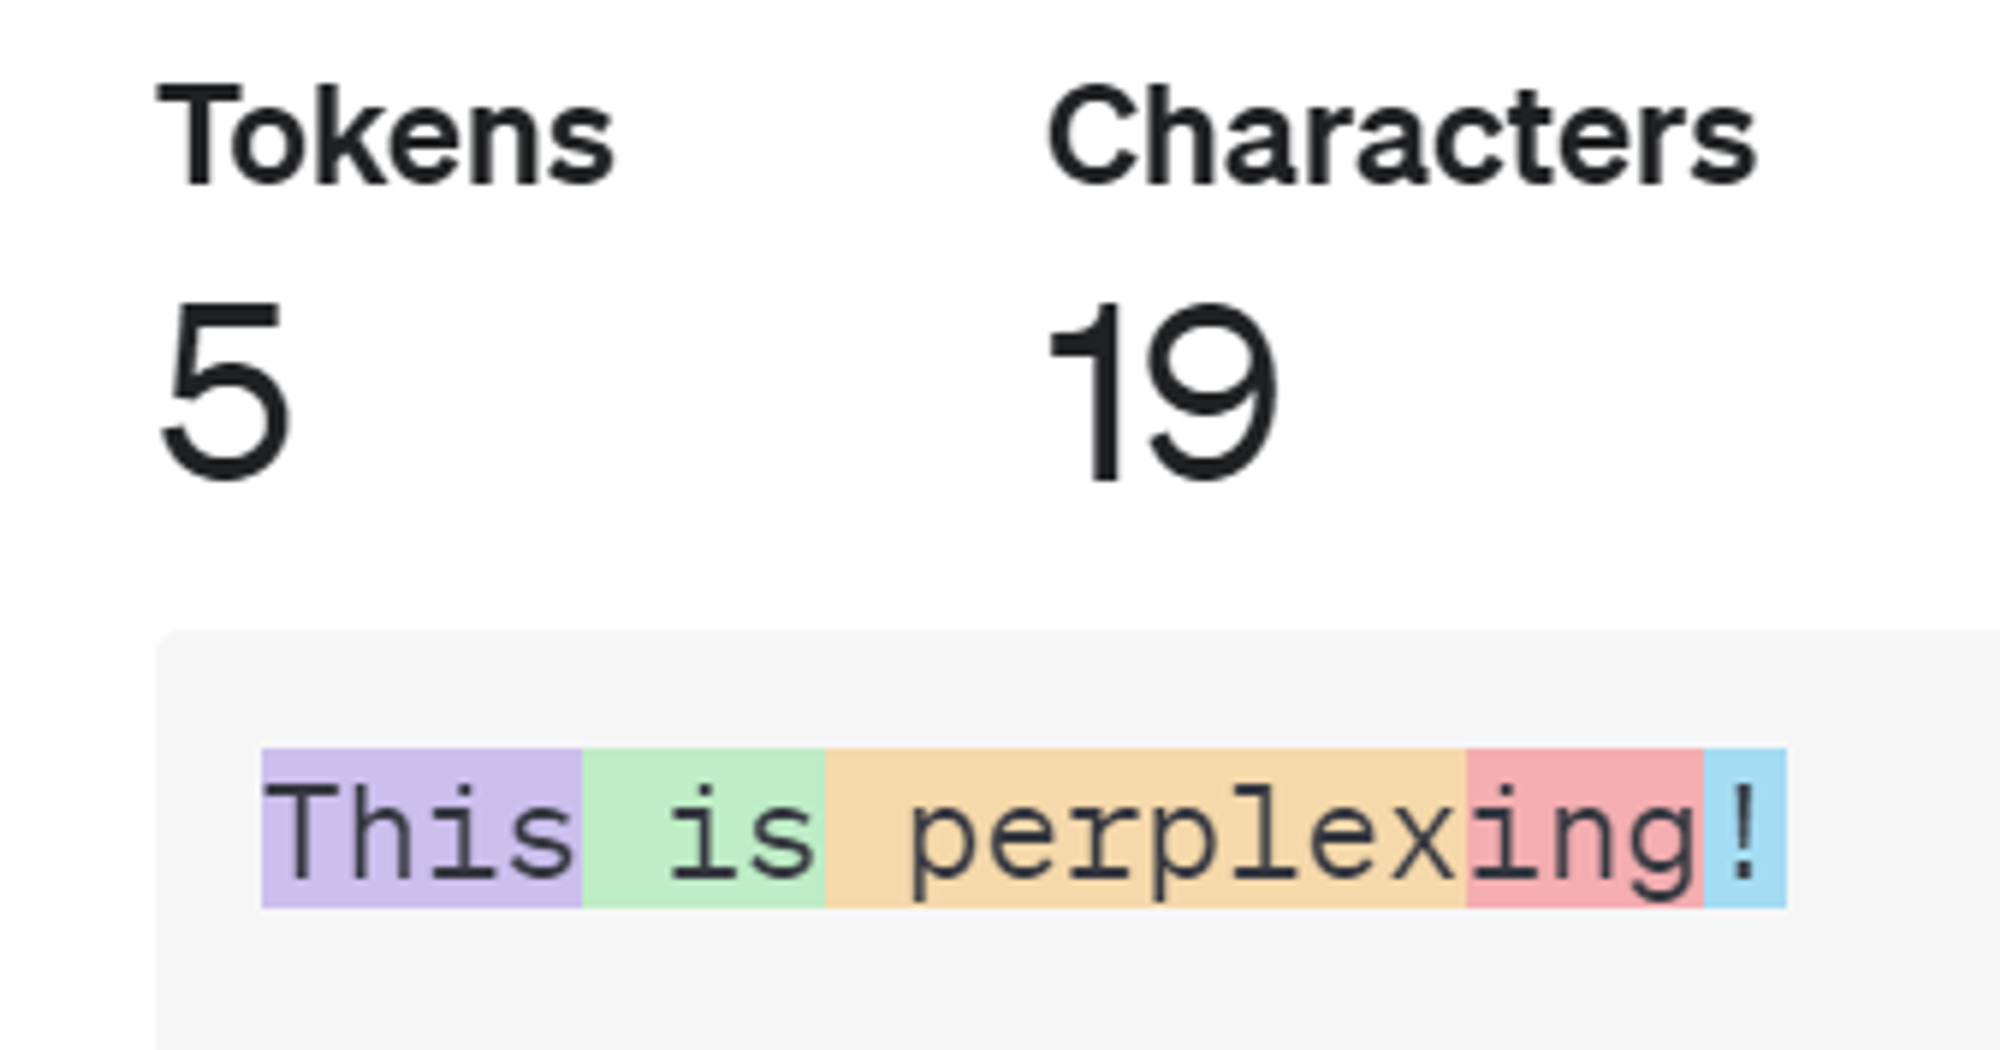
\includegraphics[width=0.35\textwidth]{images/tiktoken}
    \caption{Example of applying the tiktoken tokenizer to a sentence.}
    \label{fig:tiktoken}
\end{SCfigure}

Subword tokenization with very large dictionaries can be counter-intuitive at times: for example, common digits such as $52$ have their unique token, while digits like $2512$ can be split into a “251” token and a “2” token. For applications where processing numbers is important, specialized numerical tokenizers can be applied \cite{golkar2023xval}. In general, visualizing the tokenization process is always important to debug the models' behaviour.

After the tokenization step, the tokens must be \textbf{embedded} into vectors to be used as inputs for a CNN. A simple one-hot encoding strategy here works poorly, since vocabularies are large and the resulting vectors would be significantly sparse. Instead, we have two alternative strategies: the first is to use \textit{pretrained} networks that perform the embedding for us; we will consider this option later on, when we introduce transformers. In order to build some intuition for it, we consider here the second alternative, \textit{training} the embeddings together with the rest of the network.

Suppose we fix an embedding dimension $e$ as a hyper-parameter. Since the size $n$ of the dictionary is also fixed, we can initialize a matrix of embeddings $\mathbf{E} \sim (n, e)$. We now define a look-up operation that replaces each integer with the corresponding row in $\mathbf{E}$. Denoting by $x$ the sequence of IDs we have:

\vspace{1em}
$$
\text{LookUp}(x) =\mathbf{X} = \begin{bmatrix}   \eqnmarkbox[drawred]{node}{\mathbf{E}_{x_1}} \\\mathbf{E}_{x_2} \\ \vdots  \\\mathbf{E}_{x_{m}}\end{bmatrix}
$$
\annotate[yshift=1em]{above,right}{node}{Row $x_1$ in the embedding matrix}

\begin{SCfigure}
    \centering
    \hspace{1em}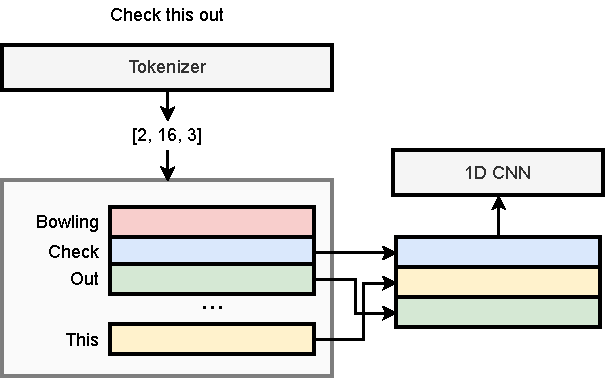
\includegraphics[width=0.6\textwidth]{images/trainable_embeddings-Page-2}
    \caption{A lookup table to convert a sequence of tokens' IDs to their curresponding embeddings: the input is a list, the output is a matrix. The embeddings (shown inside the box) can be trained together with all the other parameters via gradient descent. We assume the size of the vocabulary is $n=16$.}
    \label{fig:custom_embeddings}
\end{SCfigure}

\begin{mypy}{A 1D CNN with trainable embeddings. $n$ is the size of the dictionary, $e$ is the size of each embedding. We use two convolutional layers with $32$ and $64$ output channels. The shape of the output for each operation in the forward pass is shown as a comment.}{code:custom_embeddings}
class TextCNN(nn.Module):
  def __init__(self, n, e):
    super().__init__()
    self.emb = nn.Embedding(n, e)
    self.conv1 = nn.Conv1d(e, 32, 5, padding='same')
    self.conv2 = nn.Conv1d(32, 64, 5, padding='same')
    self.head = nn.Linear(64, 10)

  def forward(self, x):      # (*, m)
    x = self.emb(x)          # (*, m, e)
    x = x.transpose(1, 2)    # (*, e, m)
    x = relu(self.conv1(x))  # (*, 32, m)
    x = max_pool1d(x, 2)     # (*, 32, m/2)
    x = relu(self.conv2(x))  # (*, 64, m/2)
    x = x.mean(2)            # (*, 64)
    return self.head(x)      # (*, 10)
\end{mypy}

The resulting input matrix $\mathbf{X}$ will have shape $(m, e)$, where $m$ is the length of the sequence. We can now apply a generic 1D convolutional model for, e.g., classifying the text sequence:
%
$$
\hat{y}=\text{CNN}(\mathbf{X})
$$
%
This model can be trained in a standard way depending on the task, except that gradient descent will be performed jointly on the parameters of the model and the embedding matrix $\mathbf{E}$. This is shown visually in Figure \ref{fig:custom_embeddings}, and an example of model's definition is given in Box \ref{code:custom_embeddings}.

This idea is extremely powerful, especially because in many cases we find that the resulting embeddings can be manipulated algebraically as vectors, e.g., by looking at the closest embeddings in an Euclidean sense to find “semantically similar” words or sentences. This idea is at the core of the use of differentiable models in many sectors that necessitate retrieval or search of documents.

\begin{supportbox}{Differentiable models and embeddings}
Once again, the idea of embedding is very general: any procedure that converts an object into a vector with algebraic characteristics is an embedding. For example, the output of the backbone of a trained CNN after global pooling can be understood as a high-level embedding of the input image, and it can be used to retrieve “similar” images by comparing it to all other embeddings.
\end{supportbox}

\subsection{Dealing with long sequences}

Many of the sequences described before can be very long. In this case, the locality of convolutional layers can be a drawback, because we need a linearly increasing number of layers to process larger and larger receptive fields. We will see in the next chapters that other classes of models (e.g., transformers) can be designed to solve this problem. For now we remain in the realm of convolutions and we show one interesting solution, called \textbf{dilated} (or \textbf{atrous}, from the French \textit{à trous}) convolutions, popularized in the WaveNet model for speech generation \cite{oord2016wavenet}.

We introduce an additional hyper-parameter called the \textbf{dilation rate}. A convolution with dilation rate of $1$ is a standard convolution. For a dilation rate of $2$, we modify the convolution operation to select elements for our patch by skipping one out of two elements in the sequence. Similarly, for a dilation rate of $4$, we skip three elements over four, etc. We stack convolutional layers with exponentially increasing dilation rates, as shown in Figure \ref{fig:convolution_with_dilation}.

\begin{SCfigure}
    \centering
    \hspace{1em}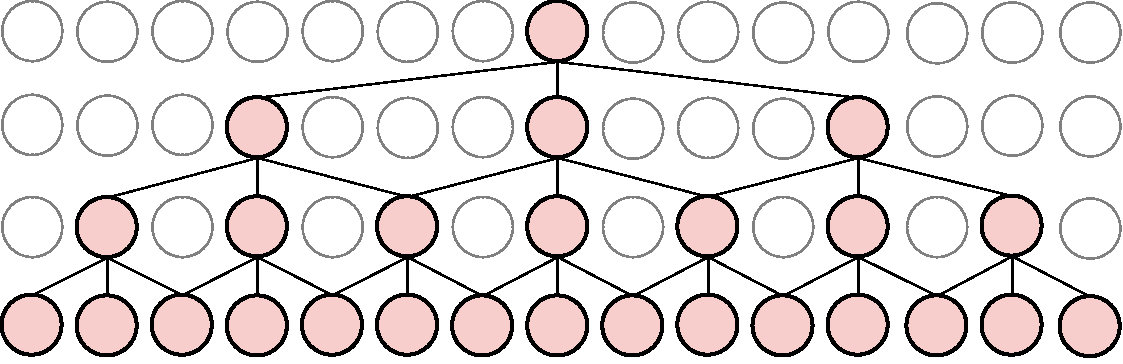
\includegraphics[width=0.55\textwidth]{images/convolution_with_dilation}
    \caption{Convolutional layers with increasing dilation rates. Elements selected for the convolution are in red, the others are greyed out. We show the receptive field for a single output element.}
    \label{fig:convolution_with_dilation}
\end{SCfigure}

The number of parameters does not change, since the number of neighbors remain constant irrespective of the dilation rate. However, it is easy to show that the resulting receptive field in this case grows \textit{exponentially fast} in the number of layers.

\section{Forecasting and causal models}
\subsection{Forecasting sequences}

One important aspect of working with sequences is that we can build a model to predict future elements, e.g., energy prices, turbulence flows, call center occupations, etc. Predicting tokens is also the fundamental building block for large language models and other recent breakthroughs. In a very broad sense, much of the current excitement around neural networks revolves around the question of how much a model can be expected to infer from next-token prediction on large corpora of text, and how much this setup can be replicated across different modalities (e.g., videos) and dynamics \cite{wang2023scientific}. Formally, predicting the next element of a sequence is called \textbf{forecasting} in statistics and time series analysis. From now on, to be consistent with modern literature, we will use the generic term \textbf{token} to refer to each element of the sequence, irrespective of whether we are dealing with an embedded text token or a generic vector-valued input.

\begin{supportbox}{Stationarity and forecasting}
Just like text processing, forecasting real-world time series has a number of associated problems (e.g., the possible non-stationarity of the time series, trends and seasonalities) that we do not consider here.\footnote{\url{https://filippomb.github.io/python-time-series-handbook/}} In practice, audio, text, and many other sequences of interest can be considered stationary and do not need special preprocessing. Like for text, for very large forecasting datasets and correspondingly large models, the impact of preprocessing tend to diminish \cite{ansari2024chronos}.
\end{supportbox}

The reason forecasting is an important problem is that we can train a forecasting model by just having access to a set of sequences, with no need for additional target labels: in modern terms, this is also called a \textbf{self-supervised learning} task, since the targets can be automatically extracted from the inputs. 

To this end, suppose we fix a user-defined length $t$, and we extract all possible subsequences of length $t$ from the dataset (e.g., with $t=12$, all consecutive windows of $12$ elements, or all sentences composed of $12$ tokens, etc.). In the context of LLMs, the size of the input sequence is called the \textbf{context} of the model. We associate to each subsequence a target value which is the next element in the sequence itself. Thus, we build a set of pairs $(\mathbf{X}, \mathbf{y}), \mathbf{X} \sim (t, c) \,,\, y \sim (c)$ and our forecasting model is trained in a supervised way over this dataset:
%
$$
f(\mathbf{X})\approx \mathbf{y}
$$
%
Note that a standard 1D convolutional model can be used as forecasting model, trained with either mean-squared error (for continuous time series) or cross-entropy (for categorical sequences, such as text). While the model is trained to predict a single step-ahead, we can easily use it to generate as many steps as we want by what is called an \textbf{autoregressive} approach, meaning that the model is predicting (\textit{regressing}) on its own outputs. Suppose we predict a single step, $\widehat{\mathbf{y}} = f(\mathbf{X})$, and we create a “shifted” input by adding our predicted value to the input (removing the first element to avoid exceeding $t$ elements):

\begin{equation}
\mathbf{X}^\prime = \begin{bmatrix} \eqnmarkbox[drawred]{node}{\mathbf{X}_{2:t}} \\ \eqnmarkbox[drawgreen]{node2}{\widehat{\mathbf{y}}} \end{bmatrix}
\label{eq:shifted_input}
\end{equation}
\annotate[yshift=1em]{above,right}{node}{Window of $t-1$ input elements}
\annotate[yshift=-1em]{below,right}{node2}{Predicted value at time $t+1$}

\vspace{1.5em}
\begin{supportbox}{Forecasting discrete sequences}
For a continuous time series this is trivial. For a time series with discrete values, $f$ will return a probability vector over the possible values (i.e., possible tokens), and we can obtain $\widehat{\mathbf{y}}$ by taking its $\arg\max$, i.e., the token associated to the highest probability. Alternatively, we can sample a token proportionally to the predicted probabilities: see Section \ref{subsec:probabilistic_formulation_generative_models}.
\end{supportbox}

We can now run $f(\mathbf{X}^\prime)$ to generate the next input value in the sequence, and so on iteratively, by always updating our buffered input in a FIFO fashion. This approach is extremely powerful, but it requires us to fix a priori the input sequence length, which limits its applicability. To overcome this limitation, we need only a minor modification to our models.

\subsection{Causal models} \addclock

Suppose we only have available a short sequence of 4 elements collected into a matrix $\mathbf{X} \sim (4, c)$, but we have trained a forecasting model on longer sequences with $t=6$. In order to run the model on the shorter sequence, we can zero-pad the sequence with two zero vectors $\mathbf{0}$ at the beginning, but these will be interpreted by the model as actual values of the time series unless we mask its operations. Luckily, there is a simpler and more elegant approach in the form of \textbf{causal} models.

\begin{definition}[Causal layer] \addbottle
A layer $\mathbf{H} = f(\mathbf{X})$ is \textbf{causal} if $\mathbf{H}_i = f(\mathbf{X}_{:i})$, i.e., the value corresponding to the $i$-th element of the sequence depends only on elements “from its past”.
\end{definition}

A model composed only of causal layers will, of course, be causal itself. For example, a convolutional layer with kernel size $1$ is causal, since each element is processed considering only itself. However, a convolutional layer with kernel size $3$ is not causal, since it is processed considering in addition one element to the left and one element to the right. We can convert any convolution into a causal variant by partially zero masking the weights corresponding to non-causal connections:
%
$$
\mathbf{h}_i=\phi\left(\left[\eqnmarkbox[drawred]{node}{\mathbf{W}\odot \mathbf{M}}\right]\text{vect}(P_{k}(i)) + \mathbf{b}\right)
$$
\annotate[yshift=-1em]{below,right}{node}{Masked weight matrix}

where $M_{ij} = 0$ if the weight corresponds to an element in the input such that $j > i$, $1$ otherwise. Causal 1D convolutions can be combined with dilated kernels to obtain autoregressive models for audio, such as in the WaveNet model \cite{oord2016wavenet} - see Figure \ref{fig:causal_convolutions} for an example.

\begin{SCfigure}
    \centering
    \hspace{1em}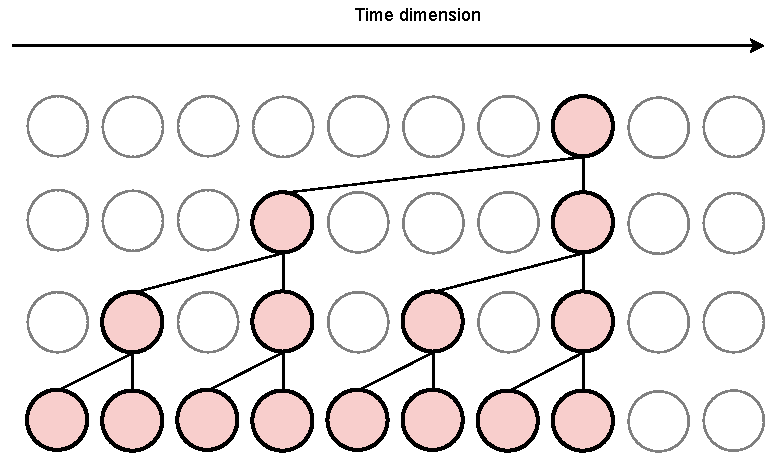
\includegraphics[width=0.5\textwidth]{images/causal_convolutions}
    \caption{Overview of a 1D \textit{causal} convolutional layer with (original) kernel size of $3$ and exponentially increasing dilation rates. Zeroed out connections are removed, and we show the receptive field for a single output element.}
    \label{fig:causal_convolutions}
\end{SCfigure}

Masking is easier to understand in the case of a single channel, in which case $\mathbf{M}$ is simply a lower-triangular binary matrix. The masking operation effectively reduces the number of parameters from $(2k+1)cc^\prime$ to $(k+1)cc^\prime$. 

By stacking several causal convolutional layers, we can obtain a causal 1D model variant. Suppose we apply it on our input sequence, with a model that has no max-pooling operations. In this case, the output sequence has the same length as the input sequence:
%
$$
\widehat{\mathbf{Y}} = f_{\text{causal}}(\mathbf{X})
$$
%
In addition, any element in the output only depends on input elements in the same position or preceding it. Hence, we can define a more sophisticated forecasting model by predicting a value \textit{for each element of the input sequence}. Practically, consider now a matrix output defined as:
%
$$
\mathbf{Y} = \begin{bmatrix} \mathbf{X}_{2:t} \\\mathbf{y} \end{bmatrix}
$$


\begin{figure}[t]
    \centering
    \begin{subfigure}[b]{0.45\textwidth}
    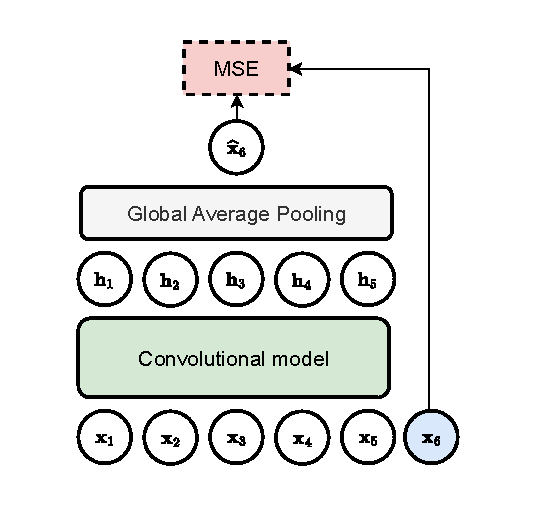
\includegraphics[width=1.0\textwidth]{images/forecasting-Page-1}
    \caption{Non-causal model}
    \label{fig:forecasting_a}
    \end{subfigure}
    \begin{subfigure}[b]{0.48\textwidth}
    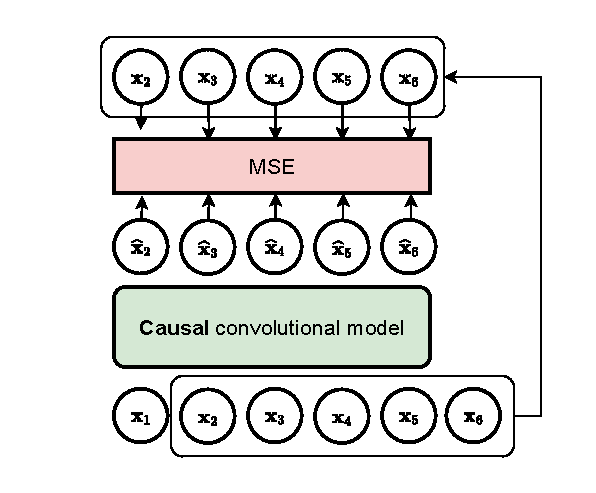
\includegraphics[width=1.0\textwidth]{images/forecasting-Pagina-2}
    \caption{Causal model}
    \label{fig:forecasting_b}
    \end{subfigure}
    \caption{Comparison between (a) a non-causal model for forecasting (predicting only a single element for the entire input sequence) and (b) a causal model trained to predict one output element for each input element in the sequence.}
    \label{fig:forecasting}
\end{figure}


This is similar to the shifted input from \eqref{eq:shifted_input}, except that we are adding the true value as last element of the sequence. We can train this model by minimizing a loss on all elements, e.g., a mean-squared error:
%
\begin{equation}
l(\widehat{\mathbf{Y}},\mathbf{Y})=\lVert \widehat{\mathbf{Y}} - \mathbf{Y} \rVert^2=\sum_{i=1}^t \eqnmarkbox[drawred]{node}{\lVert \widehat{\mathbf{Y}}_i - \mathbf{Y}_i \rVert^2}
\label{eq:mse_forecasting_multiple}
\end{equation}
\annotate[yshift=-1em]{below,right}{node}{Loss when predicting $\mathbf{X}_{i+1}$}

We simultaneously predict the second element based on the first one, the third one based on the first two, etc. For a single input window, we have $t$ separate loss terms, greatly enhancing the gradient propagation. A comparison between the two approaches is shown in Figure \ref{fig:forecasting}: in Figure \ref{fig:forecasting_a} we show a non-causal convolutional model trained to predict the next element in the sequence, while in Figure \ref{fig:forecasting_b} we show a causal model trained according to \eqref{eq:mse_forecasting_multiple}.

\begin{figure}
    \centering
    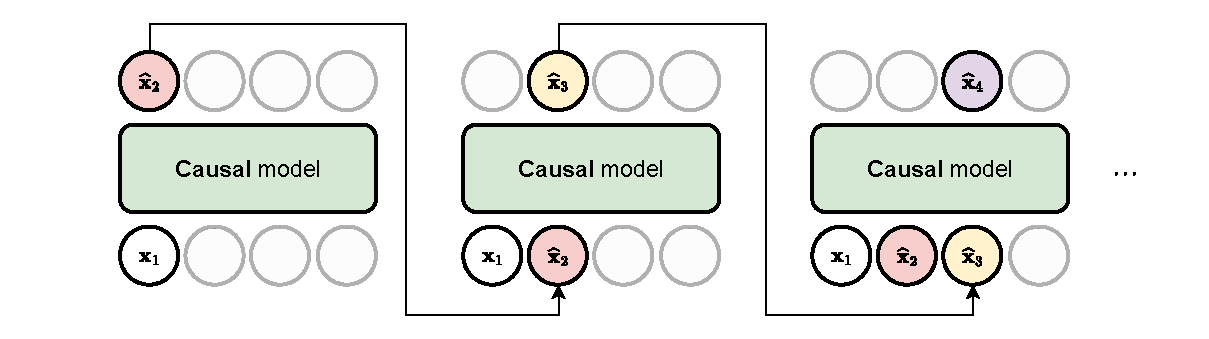
\includegraphics[width=0.95\textwidth]{images/forecasting-Pagina-3}
    \caption{Inference with a causal CNN, generating a sequence step-by-step in an autoregressive way. Unused input tokens are greyed out. Generated tokens are colored with different colors to distinguish them.}
    \label{fig:forecasting_autoregressive}
\end{figure}

More importantly, we can now use the model in an autoregressive way with any sequence length up to the maximum length of $t$. This can be seen easily with an example. Suppose we have $t=4$, and we have observed two values $\mathbf{x}_1$ and $\mathbf{x}_2$. We call the model a first time by zero-padding the sequence to generate the third token:
%
$$
\begin{bmatrix} - \\  {\color{drawred}\widehat{\mathbf{x}}_3} \\ - \\ - \end{bmatrix} =f\left( \begin{bmatrix} \mathbf{x}_1 \\ \mathbf{x}_2 \\ \mathbf{0} \\ \mathbf{0} \end{bmatrix} \right)
$$
%
We are ignoring all output values except the second one (in fact, the third and fourth outputs are invalid due to the zero-padding). We add $\widehat{\mathbf{x}}_3$ to the sequence and continue calling the model autoregressively (we show in color the predicted values):



$$
\begin{bmatrix} - \\  - \\ {\color{drawgreen}\widehat{\mathbf{x}}_4} \\ - \end{bmatrix} =f\left( \begin{bmatrix} \mathbf{x}_1 \\ \mathbf{x}_2 \\ {\color{drawred}\widehat{\mathbf{x}}_3} \\ \mathbf{0} \end{bmatrix} \right) \;,\;\begin{bmatrix} - \\  - \\ - \\ {\color{drawblue}\widehat{\mathbf{x}}_5} \end{bmatrix} =f\left( \begin{bmatrix} \mathbf{x}_1 \\ \mathbf{x}_2 \\ {\color{drawred}\widehat{\mathbf{x}}_3} \\ {\color{drawgreen}\widehat{\mathbf{x}}_4} \end{bmatrix} \right) \;,\; \begin{bmatrix}  - \\ - \\ - \\{\color{orange}\widehat{\mathbf{x}}_6}  \end{bmatrix} =f\left( \begin{bmatrix} \mathbf{x}_2 \\ {\color{drawred}\widehat{\mathbf{x}}_3} \\ {\color{drawgreen}\widehat{\mathbf{x}}_4} \\ {\color{drawblue}\widehat{\mathbf{x}}_5} \end{bmatrix}  \right) \; \ldots
$$

In the last step we removed one of the original inputs to keep the constraint on the size of the input. This is also shown in Figure \ref{fig:forecasting_autoregressive}. Note that the model is trained only on real values, not on its own predictions: this is called \textbf{teacher forcing}. A variant of teacher forcing is to progressively replace some of the values in the mini-batches with values predicted by the model, as training proceeds and the model becomes more accurate. 

Causal autoregressive models are especially interesting in the case of text sequences (where we only have a single channel, the index of the tokens), since we can start from a single [BOS] token representing the beginning of the sequence and generate text sentences from scratch, or \textit{condition} the generation on a specific prompt by the user which is appended to the [BOS] token. A similar reasoning can be applied to audio models to generate speech or music \cite{oord2016wavenet}.

\section{Autoregressive and generative models}
\subsection{A probabilistic formulation of generative models}
\label{subsec:probabilistic_formulation_generative_models} \addteacup

An autoregressive model is a simple example of a \textbf{generative model}.\footnote{Remember from Chapter \ref{chap:supervised_learning} that we assume our supervised pairs $(x,y)$ come from some unknown probability distribution $p(x,y)$. By the product rule of probability we can decompose it equivalently as $p(y \mid x)p(x)$, or $p(x \mid y)p(y)$. Any model which approximates $p(x)$ or $p(x \mid y)$ is called \textbf{generative}, because you can use it to sample new input points. By contrast, a model that only approximates $p(y \mid x)$, like we did in the previous chapters, is called \textbf{discriminative}.} We will talk at length about other types of generative models in the next volume. For now, we provide some insights specific to autoregressive algorithms. We consider sequences with a single channel and discrete values, such as text. Autoregressive models over text tokens are the foundation of LLMs, and they can be used as the basis for multimodal architectures (Chapter \ref{chap:transformers_in_practice}).

Generative models are more naturally framed in the context of probabilities, so we begin by reframing our previous discussion with a probabilistic formalism. Denote by $\mathcal{X}$ the space of all possible sequences (e.g., all possible combinations of text tokens). In general, many of these sequences will be invalid, such as the sequence [“\textit{tt}”, “\textit{tt}”] in English. However, even very uncommon sequences may appear at least once or twice in very large corpora of text (imagine a character yelling “\textit{Scotttt!}”). 

We can generalize this by considering a probability distribution $p(x)$ over all possible sequences $x \in \mathcal{X}$. In the context of text, this is also called a \textbf{language model}. Generative modeling is the task of learning to sample efficiently from this distribution:\footnote{In this section $\sim$ is used to denote sampling from a probability distribution instead of the shape of a tensor.}
%
$$
x \sim p(x)
$$
%
To see how this connects to our previous discussion, note that by the product rule of probability we can always rewrite $p(x)$ as:
%
\begin{equation}
p(x)=\prod_ip(x_i \mid x_{:i})
\label{eq:prob_autoregressive}
\end{equation}
%
where we condition each value $x_i$ to all preceding values. If we assume that our model input length is large enough to accommodate all possible sequences, we can use a causal forecasting model to parameterize the probability distribution in \eqref{eq:prob_autoregressive}:
%
$$
p(x_i \mid x_{:i})=\text{Categorical}(x_i\mid f(x_{:i}))
$$
%
where we use a single, shared model for all time-steps. Maximum likelihood over this model is then equivalent to minimizing a cross-entropy loss over the predicted probabilities, as in Section \ref{subsec:logistic_regression}.

\subsection{Sampling in an autoregressive model}

In general, sampling from a probability distribution is non-trivial. However, for autoregressive models we can exploit the product decomposition in \eqref{eq:prob_autoregressive} to devise a simple iterative strategy:
%
\begin{enumerate}
\item Sample $x_1 \sim p(x_1)$. This is equivalent to conditioning on the empty set $p(x_1 \mid \{\})$. In practice, we always condition on an initial fixed token, such as the [BOS] token, so that our input is never empty.
\item Sample $x_2 \sim p(x_2 \mid x_1)$ by running again the network with the value we sampled at step (1), as in Figure \ref{fig:forecasting_autoregressive}.
\item Sample $x_3 \sim p(x_3 \mid x_1, x_2)$.
\item Continue until we reach a desired sequence length or until we get to an end-of-sentence token.
\end{enumerate}

We did this implicitly before by always sampling the element of highest probability:
%
$$
x_i=\underset{i}{\arg\max} \;f(x_{:i})
$$
%
However, we can also generalize this by sampling a value according to the probabilities predicted by $f$. Remember (Section \ref{sec:softmax}) that the softmax can be generalized by considering an additional temperature parameter. By varying this parameter during inference, we can vary smoothly between always taking the argmax value (very low temperature) to having an almost uniform distribution over tokens (very high temperature).

In the context of probabilistic modelling, sampling in this way from this class of models is called \textbf{ancestral sampling}, while in the context of language modelling we sometimes use the term \textbf{greedy decoding}. The use of the term “greedy” and this brief discussion is enough to highlight one potential drawback of these models: while the product decomposition of $p(x)$ is exact, greedy decoding is not guaranteed to provide a sample corresponding to high values of $p(x)$. 

To see this, note that $f$ provides an estimate of the probability for a single token, but the probability of a sequence is given by a product of many such terms. Hence, sampling a token with high (local) probability at the beginning of a sequence may not correspond to a sequence having large (global) probability as a sentence. This is easy to visualize if you imagine the choice of the first token letting the decoding stage being “stuck” in a low-probability path.

A common mitigation to this problem is \textbf{beam search} (or \textbf{beam decoding}). In beam search, in the first step we sample $k$ different elements (called the beams, with $k$ being a user-defined parameter). In the second step, for each of our $k$ beams we sample $k$ possible continuations. Out of these $k^2$ pairs, we keep only the top-$k$ values in terms of their product probability $p(x_1)p(x_2\mid x_1)$ (or, equivalently, their log probability). We continue iteratively in this way until the end of the sequence.

Viewed under this lens, sampling the most probable sequence from our autoregressive model is a combinatorial search problem (think of a tree, where for each token we expand across all possible next tokens, and so on). From the point of view of computer programming, beam search is then an example of \textbf{breadth-first} search over this tree.

\subsection{Conditional modelling}
\label{subsec:conditional_modelling}

As we mentioned earlier, in general we may not be interested so much in generating sequences from scratch, but in generating continuations of known sequences, such as a user’s question or interaction. This can be formalized by considering \textit{conditional} probability distributions in the form $p(x \mid c)$, where $c$ is the conditioning argument, such as a user’s prompt. Our previous discussion extends almost straightforwardly to this case. For example, the product decomposition is now written as:
%
$$
p(x \mid c)=\prod_ip(x_i \mid x_{:i},c)
$$
%
where we condition on the previous inputs \textit{and} the user’s context. Sampling, decoding, etc., are extended in a similar way. 

To perform conditional generation we parameterize $p(x_i \mid x_{:i},c)$ with a neural network $f(x,c)$ such that:
%
$$
p(x_i \mid x_{:i},c) \approx \text{Categorical}(x_i \mid f(x_{:i}, c))
$$ 
%
Hence, the major difference with the unconditional case is that we need a function $f(x,c)$ having two input arguments and which satisfies causality in the first argument. When working with autoregressive models, if both $x$ and $c$ are texts we can do this easily be considering $c$ as part of the input sequence and working with a single concatenated input $x^\prime = [c \Vert x]$. For example, with the user's prompt “\textit{The capital of France}”, taking for simplicity a word tokenizer we might have:\footnote{We ignore the presence of an end-of-sequence token (EOS) to stop the autoregressive generation.}
%
\begin{gather*}
f_{\text{causal}}([\text{The}, \text{capital}, \text{of}, \text{France}]) = {\color{drawred}\text{is}} \\
f_{\text{causal}}([\text{The}, \text{capital}, \text{of}, \text{France}, {\color{drawred}\text{is}}]) = {\color{drawgreen}\text{Paris}} \\
\end{gather*}
%
Hence, we can handle unconditional and conditional modelling simultaneously with a single model.\footnote{We will see in Chapter \ref{chap:transformers_in_practice} that almost any type of data can be converted into a sequence of tokens. Suppose we are generating a text sequence conditioned on an image prompt (e.g., \textbf{image captioning}). If both text and images are converted to tokens having the same embedding size, we can apply an autoregressive model by concatenating the tokens from the two input types (also called \textbf{modalities} in this context), where we view the image tokens as the conditioning set $c$.} In the next volume we will see other examples of conditional generative models in which more sophisticated strategies are needed. We will also extend upon this topic when we discuss decoder-only transformer models in Chapter \ref{chap:transformers_in_practice}.

\section*{From theory to practice}

\begin{wrapfigure}{r}{3.0cm}
\vspace{-3em}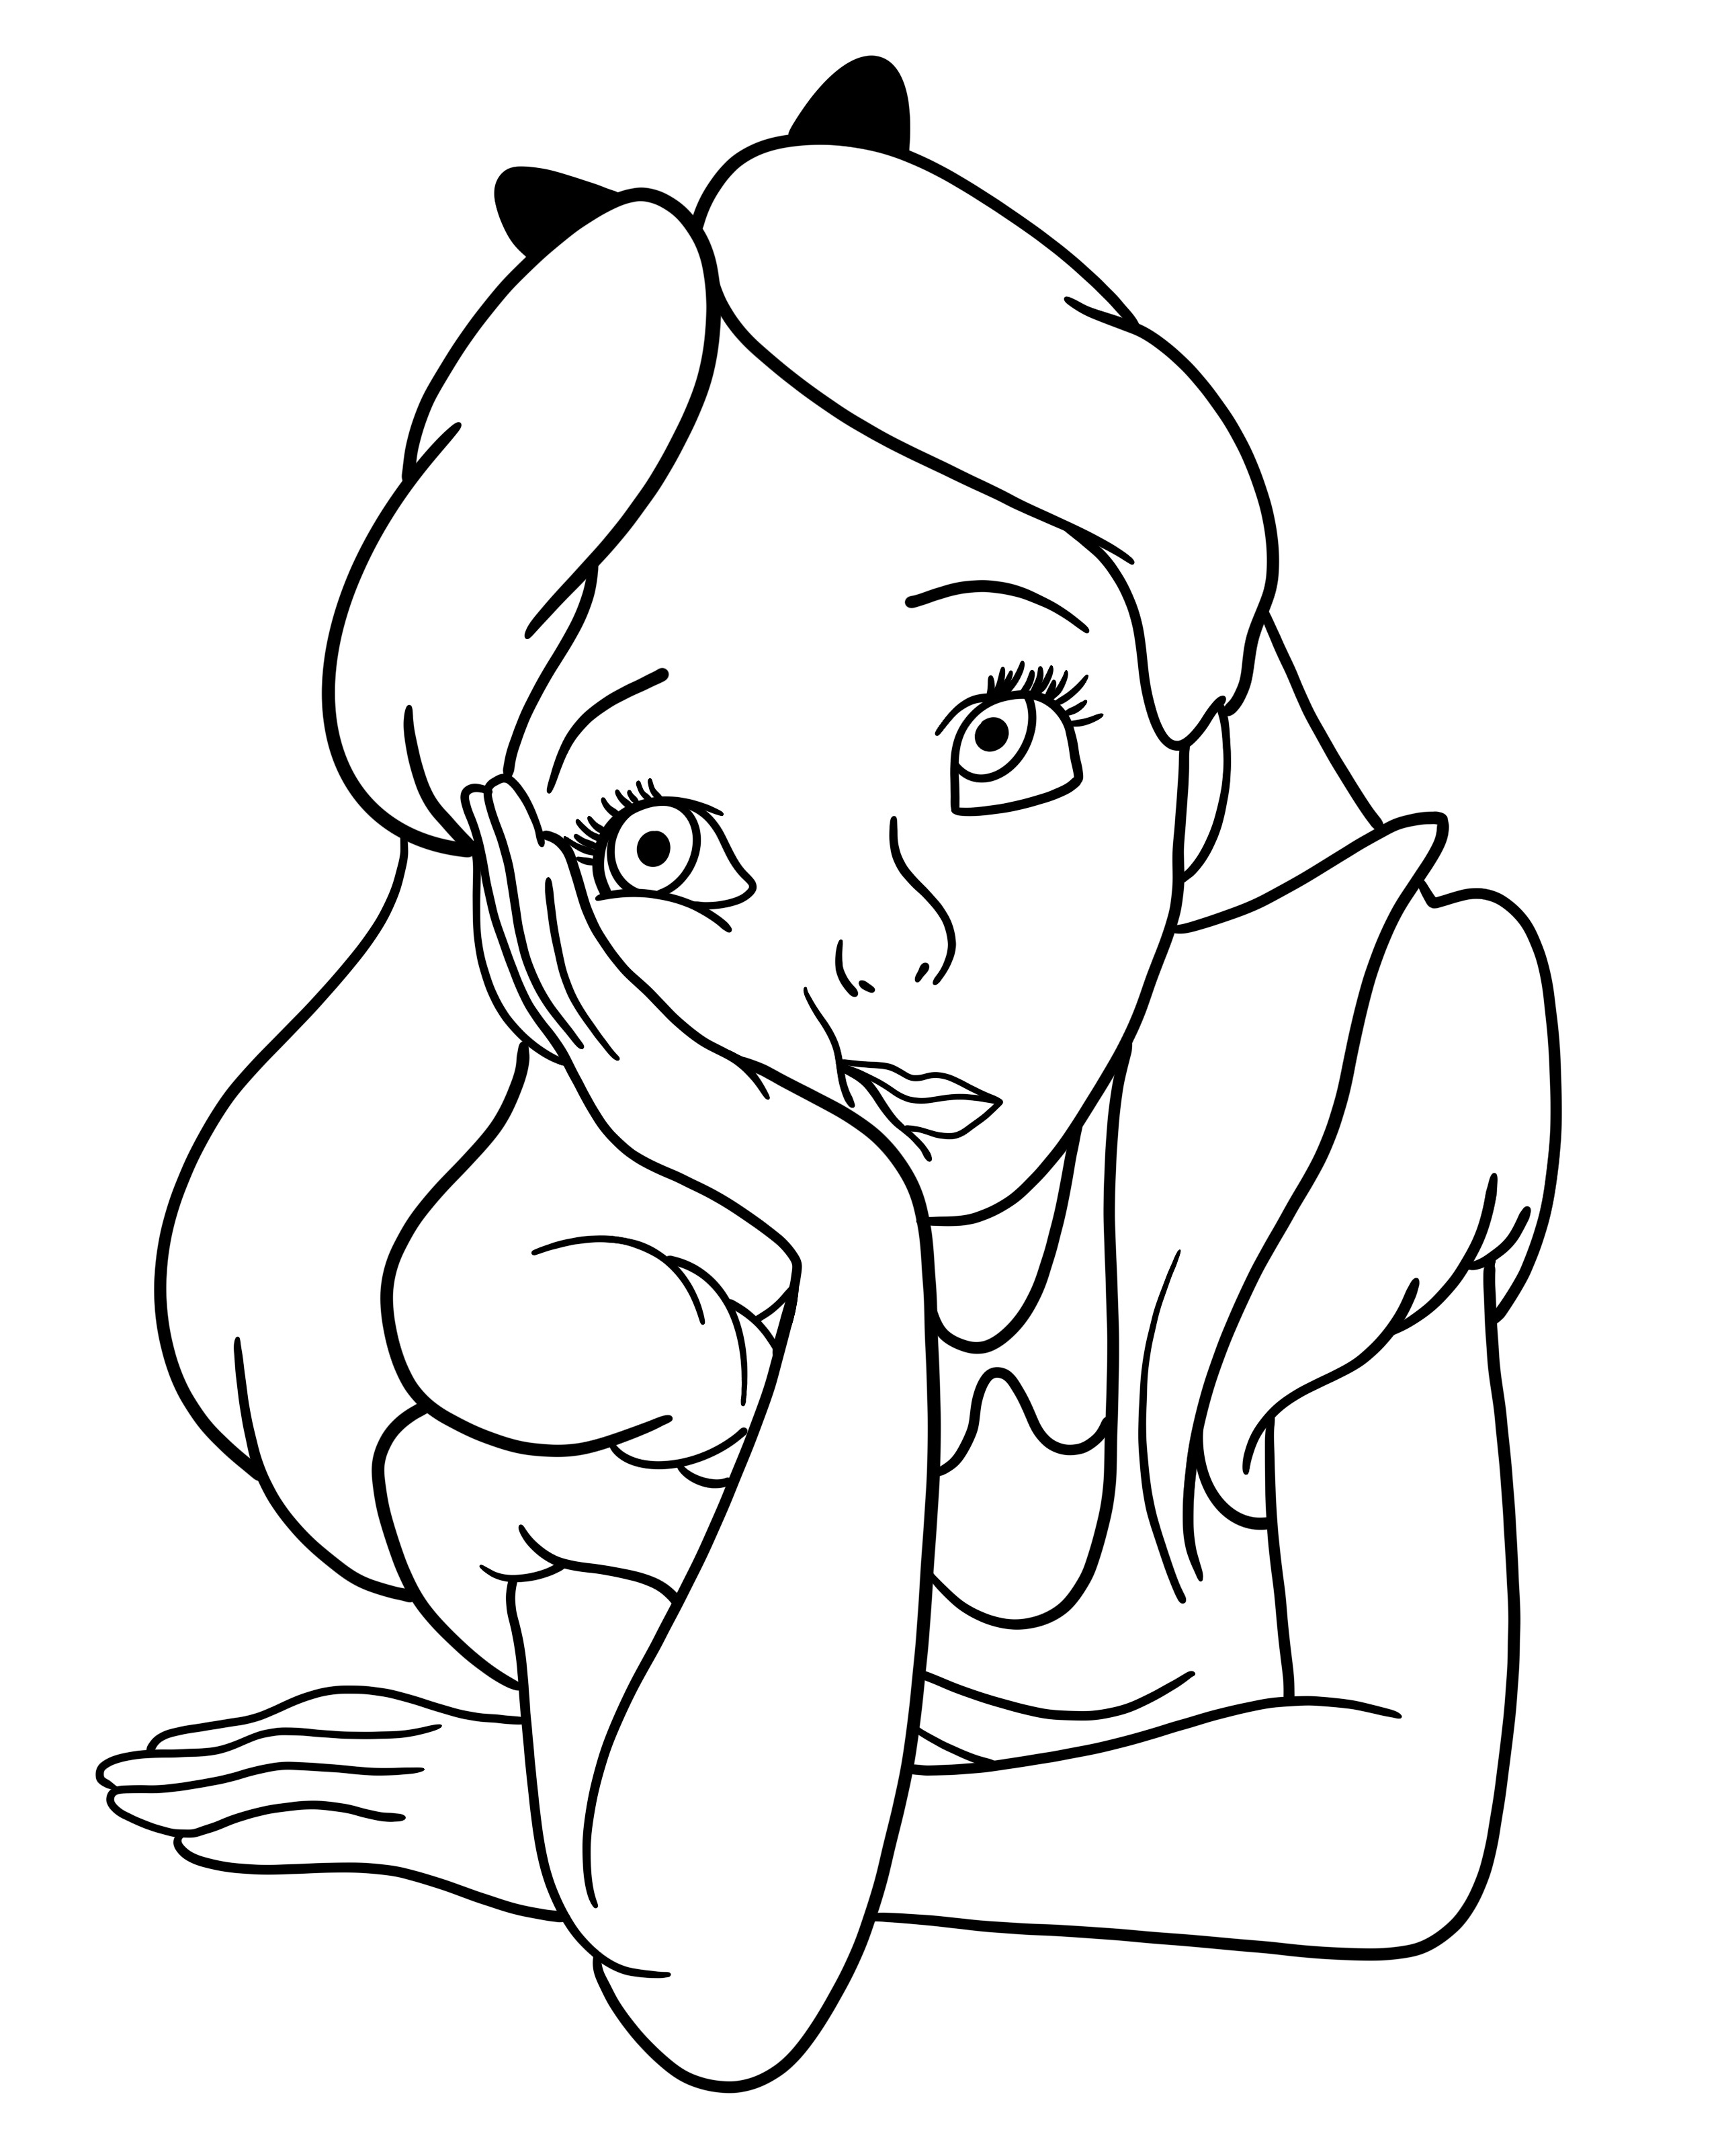
\includegraphics[width=3.0cm]{images/shutterstock_2075221579.jpg}
\vspace{-2em}
\end{wrapfigure}

Working with text data is more complex than image classification, due to many subtleties involved with tokenization, data formatting, weird characters, and variable-length sequences. PyTorch has its own text library, \texttt{torchtext}, which at the time of writing is less documented than the main library and relies on another beta library (\texttt{torchdata}) to handle the data pipelines. Thus, we ignore it here, but we invite you to check it out on your own.

Hugging Face Datasets is probably the most versatile tool in this case, as it provides a vast array of datasets and pre-trained tokenizers, which can be exported immediately to PyTorch.\footnote{See this tutorial for a guide: \url{https://huggingface.co/docs/datasets/use_dataset}.} Familiarize yourself a bit with the library before proceeding with the exercise.

\begin{enumerate}
\item Choose a text classification dataset, such as the classic IMDB dataset.\footnote{\url{https://huggingface.co/datasets/stanfordnlp/imdb}} 
\item Tokenize it to obtain a dataset of the form $(x,y)$, where $x$ is a list of integers as in \eqref{eq:list_of_indices} and $y$ is the text label.
\item Build and train a 1D CNN model similar to Box \ref{code:custom_embeddings}. Experiment a bit with the model's design to see its impact on the final accuracy.
\end{enumerate}

PyTorch does not have a quick way to make a 1D convolution causal, so we will postpone our autoregressive experiments for when we introduce transformers.\footnote{If you want to try, you can emulate a causal convolution with proper padding; see Lecture 10.2 here: \url{https://fleuret.org/dlc/}. The entire course is really good if you are looking for streamed lectures.} Training your own tokenizer is a very good didactic exercise, although it's far beyond the scope of the book. For an introduction, you can check this minimalistic BPE implementation: \url{https://github.com/karpathy/minbpe}.